\autobookmark
\begin{frame}[t]{Monte Carlo integration is embarrasingly parallel}
  \begin{columns}[T]
    \begin{column}{.5\textwidth}
      \myonly{1-2}{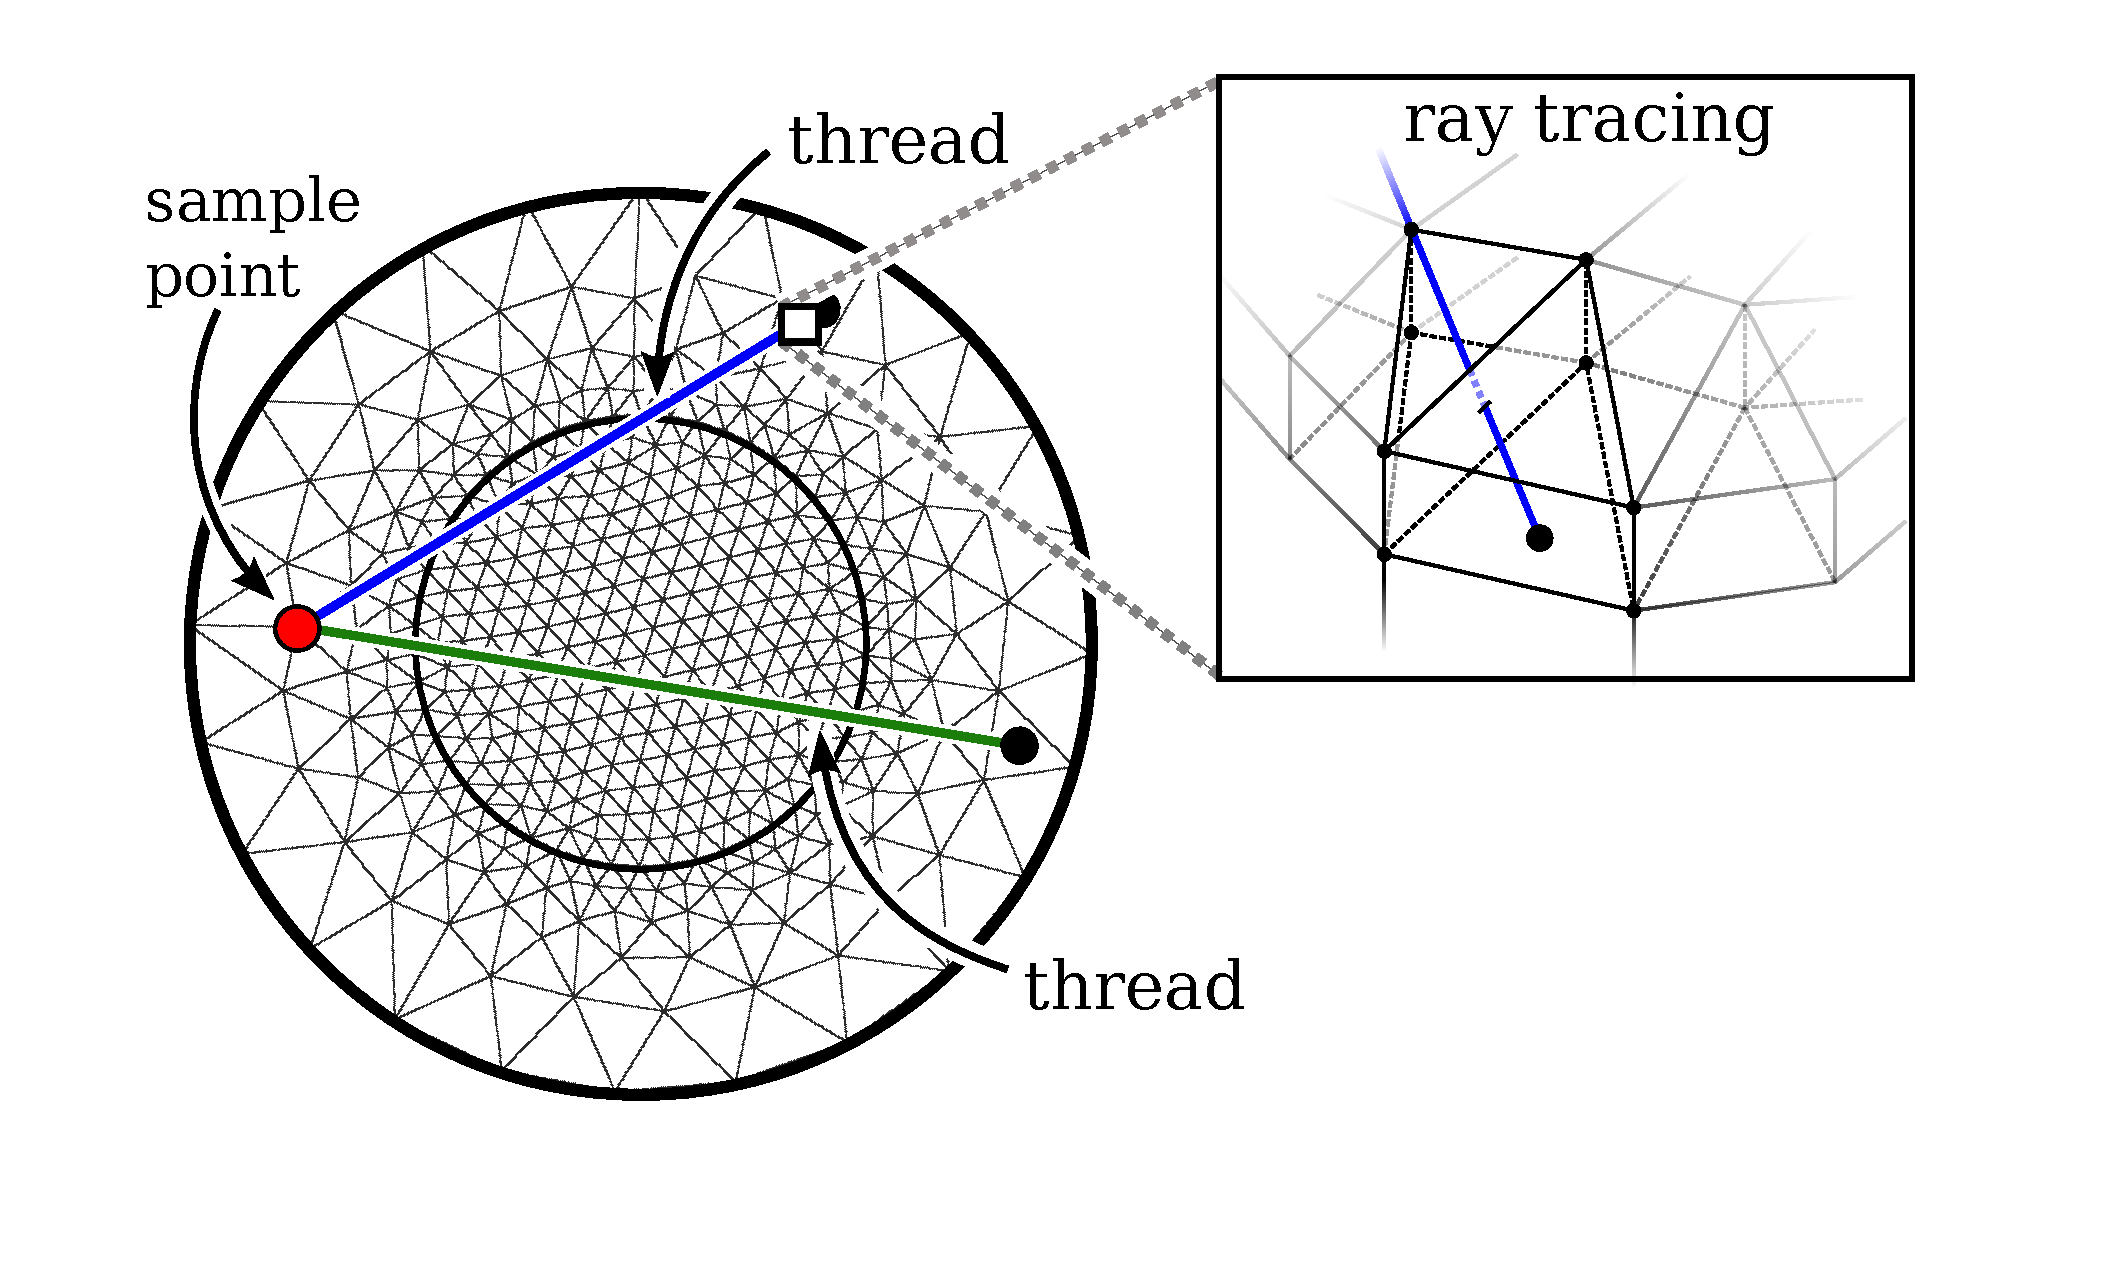
\includegraphics[height=0.55\paperheight]{graphics/monte_carlo_description_3.pdf}}
      \myonly{3-}{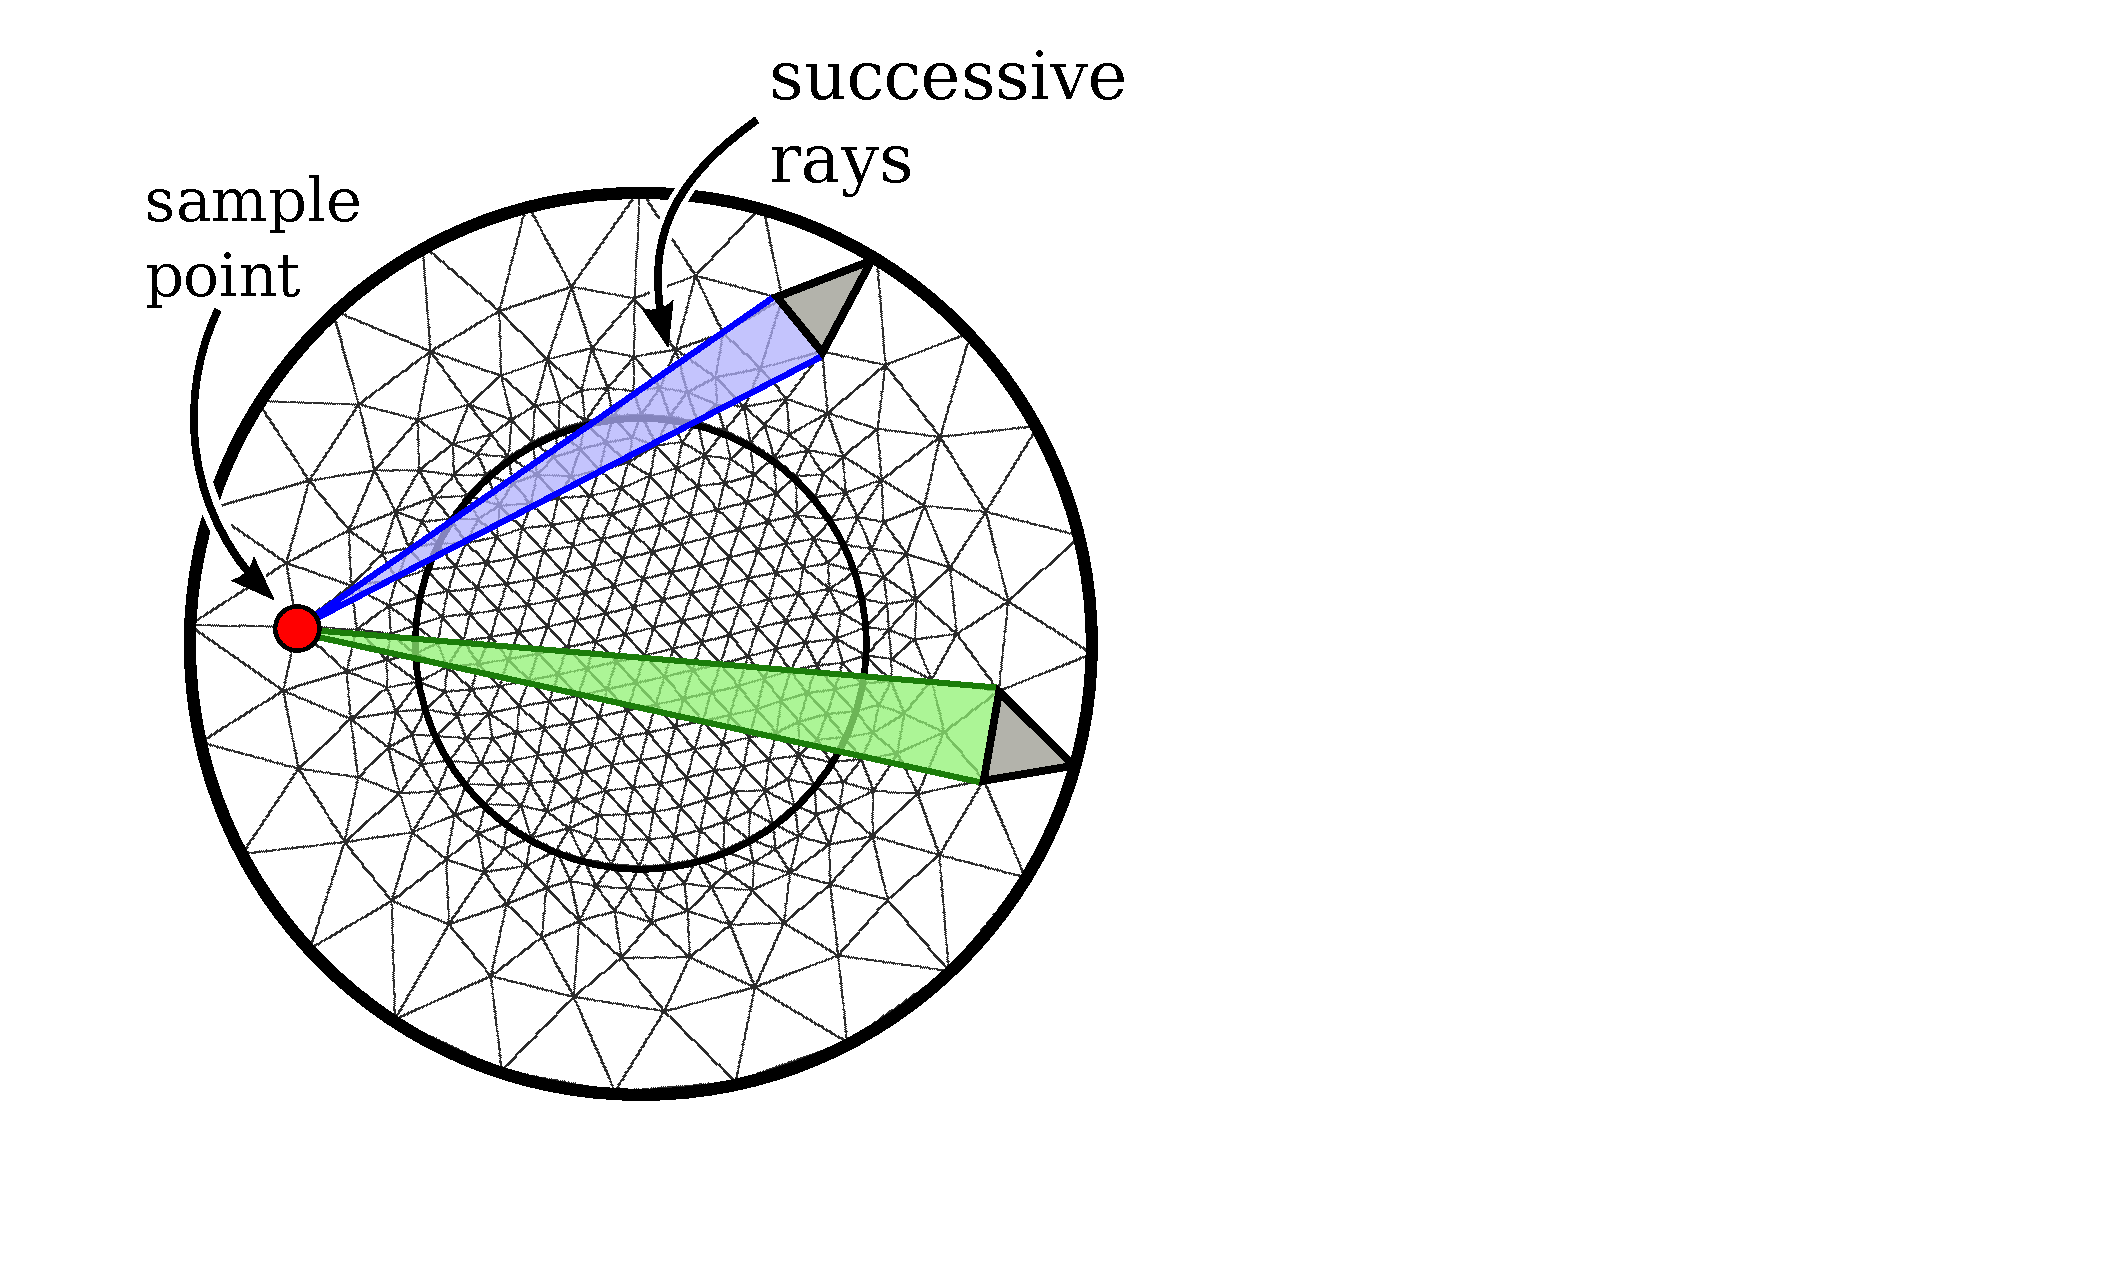
\includegraphics[height=0.55\paperheight]{graphics/monte_carlo_description_4.pdf}}
    \end{column}
    \begin{column}{.5\textwidth}
      \begin{itemize}
        \myuncover{1}{3}{
          \item Each photon is independent from the others
          \item Perfect scenario for accelerators (CUDA)
        }
        \myuncover{2}{3}{
          \item each thread computes the amplification of a single ray
        }
        \myuncover{3}{3}{
          \item successive threads start their rays in similar locations
        }
      \end{itemize}
    \end{column}
  \end{columns}
\end{frame}
